% Created by tikzDevice version 0.10.1 on 2018-01-06 23:58:38
% !TEX encoding = UTF-8 Unicode
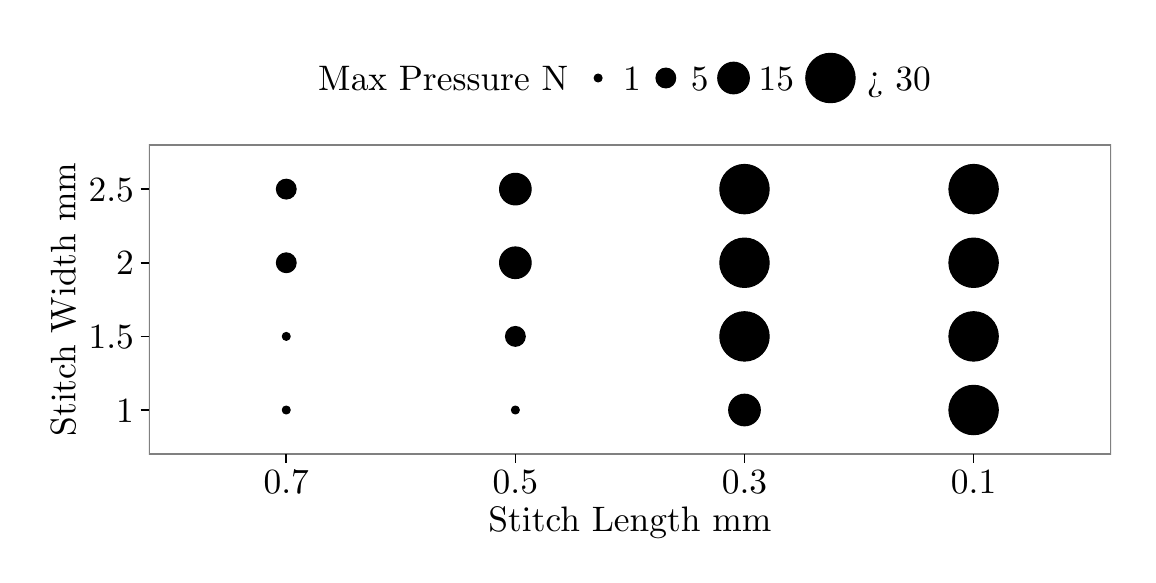
\begin{tikzpicture}[x=1pt,y=1pt]
\definecolor{fillColor}{RGB}{255,255,255}
\path[use as bounding box,fill=fillColor,fill opacity=0.00] (0,0) rectangle (397.48,190.36);
\begin{scope}
\path[clip] (  0.00,  0.00) rectangle (397.48,190.36);
\definecolor{drawColor}{RGB}{255,255,255}
\definecolor{fillColor}{RGB}{255,255,255}

\path[draw=drawColor,line width= 0.6pt,line join=round,line cap=round,fill=fillColor] (  0.00, -0.00) rectangle (397.48,202.36);
\end{scope}
\begin{scope}
\path[clip] ( 43.77, 36.23) rectangle (391.48,147.99);
\definecolor{fillColor}{RGB}{255,255,255}

\path[fill=fillColor] ( 43.77, 36.23) rectangle (391.48,147.99);
\definecolor{drawColor}{RGB}{0,0,0}
\definecolor{fillColor}{RGB}{0,0,0}

\path[draw=drawColor,line width= 0.4pt,line join=round,line cap=round,fill=fillColor] (341.81, 52.20) circle (  8.92);

\path[draw=drawColor,line width= 0.4pt,line join=round,line cap=round,fill=fillColor] (341.81, 78.80) circle (  8.92);

\path[draw=drawColor,line width= 0.4pt,line join=round,line cap=round,fill=fillColor] (341.81,105.41) circle (  8.92);

\path[draw=drawColor,line width= 0.4pt,line join=round,line cap=round,fill=fillColor] (341.81,132.02) circle (  8.92);

\path[draw=drawColor,line width= 0.4pt,line join=round,line cap=round,fill=fillColor] (259.02, 52.20) circle (  5.71);

\path[draw=drawColor,line width= 0.4pt,line join=round,line cap=round,fill=fillColor] (259.02, 78.80) circle (  8.92);

\path[draw=drawColor,line width= 0.4pt,line join=round,line cap=round,fill=fillColor] (259.02,105.41) circle (  8.92);

\path[draw=drawColor,line width= 0.4pt,line join=round,line cap=round,fill=fillColor] (259.02,132.02) circle (  8.92);

\path[draw=drawColor,line width= 0.4pt,line join=round,line cap=round,fill=fillColor] (176.23, 52.20) circle (  1.43);

\path[draw=drawColor,line width= 0.4pt,line join=round,line cap=round,fill=fillColor] (176.23, 78.80) circle (  3.57);

\path[draw=drawColor,line width= 0.4pt,line join=round,line cap=round,fill=fillColor] (176.23,105.41) circle (  5.71);

\path[draw=drawColor,line width= 0.4pt,line join=round,line cap=round,fill=fillColor] (176.23,132.02) circle (  5.71);

\path[draw=drawColor,line width= 0.4pt,line join=round,line cap=round,fill=fillColor] ( 93.44, 52.20) circle (  1.43);

\path[draw=drawColor,line width= 0.4pt,line join=round,line cap=round,fill=fillColor] ( 93.44, 78.80) circle (  1.43);

\path[draw=drawColor,line width= 0.4pt,line join=round,line cap=round,fill=fillColor] ( 93.44,105.41) circle (  3.57);

\path[draw=drawColor,line width= 0.4pt,line join=round,line cap=round,fill=fillColor] ( 93.44,132.02) circle (  3.57);
\definecolor{drawColor}{gray}{0.50}

\path[draw=drawColor,line width= 0.6pt,line join=round,line cap=round] ( 43.77, 36.23) rectangle (391.48,147.99);
\end{scope}
\begin{scope}
\path[clip] (  0.00,  0.00) rectangle (397.48,202.36);
\definecolor{drawColor}{RGB}{0,0,0}

\node[text=drawColor,anchor=base east,inner sep=0pt, outer sep=0pt, scale=  1.28] at ( 38.37, 47.79) {1};

\node[text=drawColor,anchor=base east,inner sep=0pt, outer sep=0pt, scale=  1.28] at ( 38.37, 74.40) {1.5};

\node[text=drawColor,anchor=base east,inner sep=0pt, outer sep=0pt, scale=  1.28] at ( 38.37,101.01) {2};

\node[text=drawColor,anchor=base east,inner sep=0pt, outer sep=0pt, scale=  1.28] at ( 38.37,127.61) {2.5};
\end{scope}
\begin{scope}
\path[clip] (  0.00,  0.00) rectangle (397.48,202.36);
\definecolor{drawColor}{RGB}{0,0,0}

\path[draw=drawColor,line width= 0.6pt,line join=round] ( 40.77, 52.20) --
	( 43.77, 52.20);

\path[draw=drawColor,line width= 0.6pt,line join=round] ( 40.77, 78.80) --
	( 43.77, 78.80);

\path[draw=drawColor,line width= 0.6pt,line join=round] ( 40.77,105.41) --
	( 43.77,105.41);

\path[draw=drawColor,line width= 0.6pt,line join=round] ( 40.77,132.02) --
	( 43.77,132.02);
\end{scope}
\begin{scope}
\path[clip] (  0.00,  0.00) rectangle (397.48,202.36);
\definecolor{drawColor}{RGB}{0,0,0}

\path[draw=drawColor,line width= 0.6pt,line join=round] ( 93.44, 33.23) --
	( 93.44, 36.23);

\path[draw=drawColor,line width= 0.6pt,line join=round] (176.23, 33.23) --
	(176.23, 36.23);

\path[draw=drawColor,line width= 0.6pt,line join=round] (259.02, 33.23) --
	(259.02, 36.23);

\path[draw=drawColor,line width= 0.6pt,line join=round] (341.81, 33.23) --
	(341.81, 36.23);
\end{scope}
\begin{scope}
\path[clip] (  0.00,  0.00) rectangle (397.48,202.36);
\definecolor{drawColor}{RGB}{0,0,0}

\node[text=drawColor,anchor=base,inner sep=0pt, outer sep=0pt, scale=  1.28] at ( 93.44, 22.02) {0.7};

\node[text=drawColor,anchor=base,inner sep=0pt, outer sep=0pt, scale=  1.28] at (176.23, 22.02) {0.5};

\node[text=drawColor,anchor=base,inner sep=0pt, outer sep=0pt, scale=  1.28] at (259.02, 22.02) {0.3};

\node[text=drawColor,anchor=base,inner sep=0pt, outer sep=0pt, scale=  1.28] at (341.81, 22.02) {0.1};
\end{scope}
\begin{scope}
\path[clip] (  0.00,  0.00) rectangle (397.48,202.36);
\definecolor{drawColor}{RGB}{0,0,0}

\node[text=drawColor,anchor=base,inner sep=0pt, outer sep=0pt, scale=  1.28] at (217.63,  8.40) {Stitch Length mm};
\end{scope}
\begin{scope}
\path[clip] (  0.00,  0.00) rectangle (397.48,202.36);
\definecolor{drawColor}{RGB}{0,0,0}

\node[text=drawColor,rotate= 90.00,anchor=base,inner sep=0pt, outer sep=0pt, scale=  1.28] at ( 17.22, 92.11) {Stitch Width mm};
\end{scope}
\begin{scope}
\path[clip] (  0.00,  0.00) rectangle (397.48,202.36);
\definecolor{fillColor}{RGB}{255,255,255}

\path[fill=fillColor] (100.70,156.52) rectangle (334.55,187.82);
\end{scope}
\begin{scope}
\path[clip] (  0.00,  0.00) rectangle (397.48,202.36);
\definecolor{drawColor}{RGB}{0,0,0}

\node[text=drawColor,anchor=base west,inner sep=0pt, outer sep=0pt, scale=  1.28] at (104.97,167.76) {Max Pressure N};
\end{scope}
\begin{scope}
\path[clip] (  0.00,  0.00) rectangle (397.48,202.36);
\definecolor{drawColor}{RGB}{255,255,255}
\definecolor{fillColor}{RGB}{255,255,255}

\path[draw=drawColor,line width= 0.6pt,line join=round,line cap=round,fill=fillColor] (198.90,160.79) rectangle (213.36,183.55);
\end{scope}
\begin{scope}
\path[clip] (  0.00,  0.00) rectangle (397.48,202.36);
\definecolor{drawColor}{RGB}{0,0,0}
\definecolor{fillColor}{RGB}{0,0,0}

\path[draw=drawColor,line width= 0.4pt,line join=round,line cap=round,fill=fillColor] (206.13,172.17) circle (  1.43);
\end{scope}
\begin{scope}
\path[clip] (  0.00,  0.00) rectangle (397.48,202.36);
\definecolor{drawColor}{RGB}{255,255,255}
\definecolor{fillColor}{RGB}{255,255,255}

\path[draw=drawColor,line width= 0.6pt,line join=round,line cap=round,fill=fillColor] (223.37,160.79) rectangle (237.82,183.55);
\end{scope}
\begin{scope}
\path[clip] (  0.00,  0.00) rectangle (397.48,202.36);
\definecolor{drawColor}{RGB}{0,0,0}
\definecolor{fillColor}{RGB}{0,0,0}

\path[draw=drawColor,line width= 0.4pt,line join=round,line cap=round,fill=fillColor] (230.60,172.17) circle (  3.57);
\end{scope}
\begin{scope}
\path[clip] (  0.00,  0.00) rectangle (397.48,202.36);
\definecolor{drawColor}{RGB}{255,255,255}
\definecolor{fillColor}{RGB}{255,255,255}

\path[draw=drawColor,line width= 0.6pt,line join=round,line cap=round,fill=fillColor] (247.84,160.79) rectangle (262.29,183.55);
\end{scope}
\begin{scope}
\path[clip] (  0.00,  0.00) rectangle (397.48,202.36);
\definecolor{drawColor}{RGB}{0,0,0}
\definecolor{fillColor}{RGB}{0,0,0}

\path[draw=drawColor,line width= 0.4pt,line join=round,line cap=round,fill=fillColor] (255.06,172.17) circle (  5.71);
\end{scope}
\begin{scope}
\path[clip] (  0.00,  0.00) rectangle (397.48,202.36);
\definecolor{drawColor}{RGB}{255,255,255}
\definecolor{fillColor}{RGB}{255,255,255}

\path[draw=drawColor,line width= 0.6pt,line join=round,line cap=round,fill=fillColor] (278.70,160.79) rectangle (301.46,183.55);
\end{scope}
\begin{scope}
\path[clip] (  0.00,  0.00) rectangle (397.48,202.36);
\definecolor{drawColor}{RGB}{0,0,0}
\definecolor{fillColor}{RGB}{0,0,0}

\path[draw=drawColor,line width= 0.4pt,line join=round,line cap=round,fill=fillColor] (290.08,172.17) circle (  8.92);
\end{scope}
\begin{scope}
\path[clip] (  0.00,  0.00) rectangle (397.48,202.36);
\definecolor{drawColor}{RGB}{0,0,0}

\node[text=drawColor,anchor=base west,inner sep=0pt, outer sep=0pt, scale=  1.28] at (215.17,167.76) {1};
\end{scope}
\begin{scope}
\path[clip] (  0.00,  0.00) rectangle (397.48,202.36);
\definecolor{drawColor}{RGB}{0,0,0}

\node[text=drawColor,anchor=base west,inner sep=0pt, outer sep=0pt, scale=  1.28] at (239.63,167.76) {5};
\end{scope}
\begin{scope}
\path[clip] (  0.00,  0.00) rectangle (397.48,202.36);
\definecolor{drawColor}{RGB}{0,0,0}

\node[text=drawColor,anchor=base west,inner sep=0pt, outer sep=0pt, scale=  1.28] at (264.10,167.76) {15};
\end{scope}
\begin{scope}
\path[clip] (  0.00,  0.00) rectangle (397.48,202.36);
\definecolor{drawColor}{RGB}{0,0,0}

\node[text=drawColor,anchor=base west,inner sep=0pt, outer sep=0pt, scale=  1.28] at (303.27,167.76) {> 30};
\end{scope}
\end{tikzpicture}
